% ################################
\section{Úvod}

\todo{Zde vysvětlit problémovou situaci a otázky, které se budou v bakalářské/diplomové práci řešit.}

Citace \cite{abadi_tensorflow:_2016, lacey_deep_2016}.


% ################################
\section{Cíl práce}

\todo{Smysl a účel, výzkumné otázky.}


% ################################
\section{Metodika zpracování}

\todo{Cíle, hypotézy/ výzkumné otázky, způsob hledání odpovědí na výzkumné otázky včetně metodiky vlastního výzkumu/šetření, literární rešerše.}


% ################################
\section{Vlastní text práce}

\todo{TODO}

Vlastní řešení dokládá student zpravidla v několika kapitolách. Podle charakteru práce musí student uvážit, zda informace netextové povahy (data, tabulky, obrázky atd.) bude uvádět přímo v textu, nebo je zařadí až za celou práci ve formě příloh, či bude kombinovat oba způsoby. 

Více podrobností viz Metodické pokyny pro vypracování bakalářských a diplomových prací (zveřejňované formou výnosů děkana) a v kurzu MES – Metodologický seminář. 

\subsection{Podkapitola}

Vlastní text práce.

\begin{landscape}
\pagestyle{mylandscape} %Call our predefined page type

\begin{center}
{\renewcommand{\arraystretch}{1.5}%
\begin{xltabular}{1.0 \linewidth}{ % linewidth is for landscape but for center is textwidth 
 | p { 6 em } | X % 6 em je pevná šířka sloupce zde prvního
 | > { \centering\arraybackslash } X 
 | > { \centering\arraybackslash } X 
 | > { \centering\arraybackslash } X 
 | > { \centering\arraybackslash } X
 | > { \centering\arraybackslash } X
 | > { \centering\arraybackslash } X 
 | > { \centering\arraybackslash } X 
 | > { \centering\arraybackslash } X 
 | > { \centering\arraybackslash } X 
 | > { \centering\arraybackslash } X | }
\caption{Přehledová tabulka.} \label{tab:long} \\

\hline
Identifikace & Zařazení & Využití & Verifikace, validace & Zaměření & Počet agentů, rozsah&Zdrojový kód&Využití Pythonu&ODD protokol&Reálný čas&Zdroj dat\\ \hline
\endfirsthead


\multicolumn{11}{c}%

{\tablename\ \thetable{} -- pokračování z předchozí stránky} \\
\hline
Identifikace & Zařazení& Využití& Verifikace, validace & Zaměření& Počet agentů, Rozsah&Zdrojový kód&Využití Pythonu&ODD protokol&Reálný čas& Zdroj dat \\ \hline 
\endhead

\hline \multicolumn{11}{|c|}{{Pokračování na následující stránce}} \\ \hline
\endfoot

\hline
\endlastfoot
Belotti M. C. T. D. et al., 2022 
&evakuace davu
& výzkum a tvorba modelů
&validace
&indoor, outdoor
&54 agentů, koridor 3x38 metrů
&ANO
&základní kód
&NE
&NE 
&Využívá předchozí studie
\\ \hline
Couasnon et al., 2019 

&loď, evakuace
& lodní inženýři, výzkum
& NE
& indoor
& loď - 5. paluba, 180 m dlouhá, 838 agentů
& NE
& základní kód
&NE
&ANO
&Agenti a prostředí generovány Mesa
\\ \hline
Crooks Andrew et al., 2017
 
&evakuace po výbuchu
&IZS, výzkum
&ANO
&outdoor
& oblast 262 x 234 km, 22 795 866 osob, 225 906 km silnic
&uveden nefunkční odkaz
&zpracová-ní a mapování dat
&NE
&NE
& Pomocí smíšené metody syntézy použity údaje ze sčítání lidu
\\ \hline
\end{xltabular}}
\end{center}
\end{landscape}


\subsubsection{Podřazená kapitola}
Text s odkazem na obrázek \ref{figure:uhk}.


\begin{figure}[hbt!]
 	\begin{center}
    	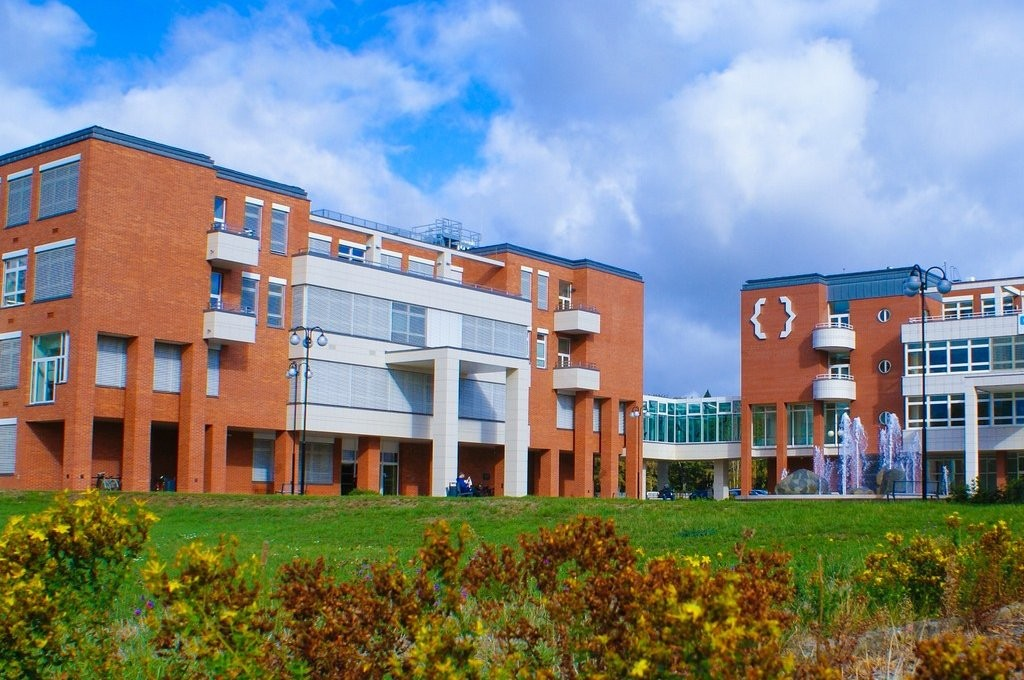
\includegraphics[width=\textwidth]{obrazky/uhk.jpg}
 	\end{center}
 	\caption{Ukázkový obrázek}
	\label{figure:uhk}
\end{figure} 


% ################################
\section{Souhrn výsledků}

\todo{Souhrn vlastních výsledků získaných v průběhu řešení problému.}

\noindent\todo{Zkratka} \Ac{DNN}


% ################################
\section{Závěry a doporučení}

\todo{Kritická diskuze nad výsledky, ke kterým autor dospěl (soulad výsledků  literaturou či předpoklady; výsledky a okolnosti, které zvláště ovlivnily předkládanou práci atd.). Je vhodné naznačit i případné další (popř. alternativní) možnosti zkoumání dané problematiky a otevřené problémy pro další studium. }
